\chapter{Bose--Hubbard 二聚体}
\label{ch:dimer}

\begin{learningobjectives}
完成本章后，读者应能：
\begin{enumerate}
  \item 从两模 Bose--Hubbard Hamiltonian 推导精确矩阵表示和 TWA 方程；
  \item 用数差与相对相位解释 Rabi 振荡、相位扩散和非线性自俘获；
  \item 在完全相同的初态与观测量下比较精确演化、平均场和 TWA；
  \item 检查 Fock 截断、Monte Carlo 误差和轨迹守恒量。
\end{enumerate}
\end{learningobjectives}

\section{连接单模与量子场的最小模型}

两模 Bose--Hubbard Hamiltonian 为
\begin{equation}
  \Hhat=-J(\had_L\ha_R+\had_R\ha_L)
  +\frac{U}{2}\sum_{\sigma=L,R}
  \had_\sigma\had_\sigma\ha_\sigma\ha_\sigma.
  \label{eq:dimer-hamiltonian}
\end{equation}
$J$ 与 $U$ 均为能量。它可以描述双阱、两个内部态的单空间模近似，或完整场论的最低两模截断。总粒子数
\begin{equation}
  \hat N=\hat n_L+\hat n_R
\end{equation}
严格守恒，但左右数差
\begin{equation}
  \hat Z=\hat n_L-\hat n_R
\end{equation}
会因隧穿而振荡。

当 $U=0$ 时，每个粒子作线性 Rabi 振荡；当 $J=0$ 时，各模式的粒子数固定，而不同数分量因相互作用积累不同相位；两者竞争时出现振幅依赖的非线性 Josephson 动力学。这个模型既可在有限 Fock 空间精确求解，也具有非平凡 TWA，因此适合系统基准。

\section{固定粒子数表象}

在固定总数 $N$ 的子空间中，基底可取
\begin{equation}
  \ket{n,N-n},\qquad n=0,1,\ldots,N.
\end{equation}
对角矩阵元为
\begin{equation}
  \mel{n,N-n}{\Hhat}{n,N-n}
  =\frac{U}{2}\left[n(n-1)+(N-n)(N-n-1)\right],
\end{equation}
相邻基矢由隧穿连接：
\begin{equation}
  \mel{n+1,N-n-1}{\Hhat}{n,N-n}
  =-J\sqrt{(n+1)(N-n)}.
  \label{eq:dimer-matrix-element}
\end{equation}
因此每个固定 $N$ 块只有 $N+1$ 维。若初态是两个相干态的直积，则总数不是固定值；精确计算需要同时包含多个 $N$ 块，或在每个模式上设置足够高的 Fock 截断。

\section{Weyl Hamiltonian 与 TWA 方程}

\cref{eq:dimer-hamiltonian} 的 Weyl 符号在略去常数后为
\begin{equation}
  H_W=-J(\alpha_L^*\alpha_R+\alpha_R^*\alpha_L)
  +\frac{U}{2}\sum_{\sigma=L,R}
  \left(|\alpha_\sigma|^4-2|\alpha_\sigma|^2\right).
  \label{eq:dimer-weyl}
\end{equation}
TWA 轨迹满足
\begin{align}
  \ii\hbar\dot\alpha_L
  &=-J\alpha_R+U(|\alpha_L|^2-1)\alpha_L,\\
  \ii\hbar\dot\alpha_R
  &=-J\alpha_L+U(|\alpha_R|^2-1)\alpha_R.
  \label{eq:dimer-twa}
\end{align}
每条连续轨迹保持 $|\alpha_L|^2+|\alpha_R|^2$ 与 $H_W$。正常排序总数估计为
\begin{equation}
  \qavg{\hat N}
  =\ensavg{|\alpha_L|^2+|\alpha_R|^2-1},
  \label{eq:dimer-total-estimator}
\end{equation}
而数差中的两个半量子互相抵消：
\begin{equation}
  \qavg{\hat Z}
  =\ensavg{|\alpha_L|^2-|\alpha_R|^2}.
\end{equation}

\section{数差与相对相位}

在高占据区写
\begin{equation}
  \alpha_L=\sqrt{\frac{N_c}{2}(1+z)}\,\ee^{-\ii\phi/2},
  \qquad
  \alpha_R=\sqrt{\frac{N_c}{2}(1-z)}\,\ee^{\ii\phi/2}.
\end{equation}
$z$ 是归一化数差，$\phi$ 是相对相位，$N_c=|\alpha_L|^2+|\alpha_R|^2$ 沿轨迹守恒。忽略与 $z,\phi$ 无关的常数后，经典 Hamiltonian 具有结构
\begin{equation}
  H_{\mathrm{rel}}
  =\frac{UN_c^2}{4}z^2
  -JN_c\sqrt{1-z^2}\cos\phi.
  \label{eq:josephson-classical-hamiltonian}
\end{equation}
数差和相对相位构成共轭变量。初始数差涨落造成不同轨迹具有不同的相位速度，这是相位扩散的直接来源。若相互作用能相对隧穿足够大，经典相图出现分离曲线和自俘获轨道；但量子隧穿、有限 $N$ 与初态宽度会使锐利的经典边界变成有限尺寸交叉。

\section{精确计算与 TWA 的同协议比较}

本章数值实验取 $\hbar=J=1$、$U=0.15$，初态为
\begin{equation}
  \ket{\psi_0}=\ket{\alpha_L=\sqrt8}\otimes\ket{\alpha_R=0}.
  \label{eq:dimer-coherent-initial}
\end{equation}
这是一项有意选择的基准：相干态 Wigner 函数可精确正抽样，因而比较不含固定粒子数态近似抽样的额外误差。代价是总粒子数服从 Poisson 分布；本结果不能直接解释为固定 $N=8$ 的实验。

精确演化在每模 $n=0,\ldots,23$ 的截断 Fock 空间中计算。截断前保留的初态范数为 $0.9999963$，随后重新归一化。TWA 使用 $20000$ 条相干态 Wigner 轨迹和四阶 Runge--Kutta 积分。比较量为
\begin{equation}
  z(t)=\frac{\qavg{\hat n_L}-\qavg{\hat n_R}}
  {\qavg{\hat n_L}+\qavg{\hat n_R}}.
  \label{eq:dimer-imbalance}
\end{equation}

\begin{figure}[htbp]
  \centering
  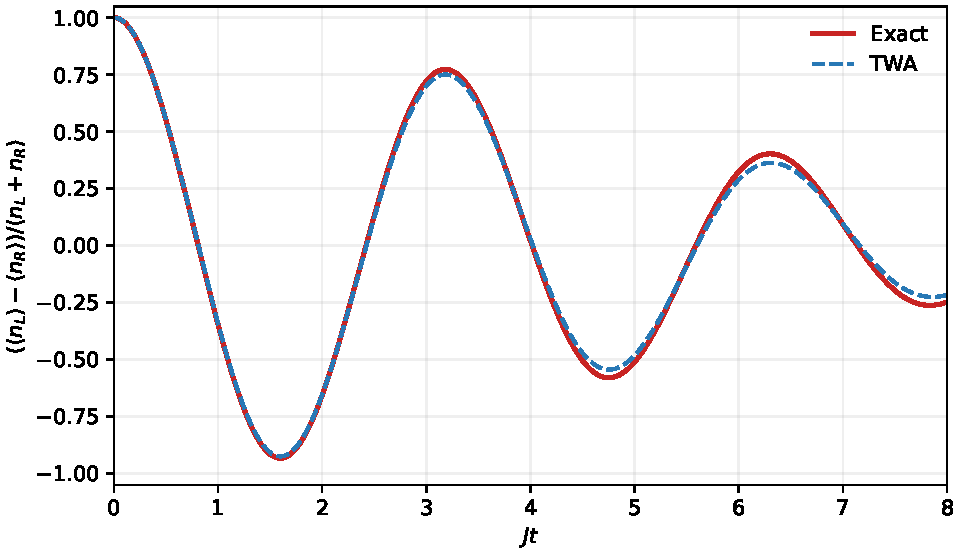
\includegraphics[width=0.82\textwidth]{figures/ch08/dimer_exact_vs_twa.pdf}
  \caption{两模 Bose--Hubbard 模型的归一化数差。红色实线为截断 Fock 空间的量子演化，蓝色虚线为 TWA。参数、初态和观测量在两种计算中完全一致。图由 \texttt{code/ch08\_dimer/dimer\_exact\_vs\_twa.py} 生成。}
  \label{fig:dimer-exact-vs-twa}
\end{figure}

在 $t\le2/J$ 的窗口内，最大数差误差为 $8.03\times10^{-3}$；整个 $0\le Jt\le8$ 窗口的均方根误差为 $2.13\times10^{-2}$。TWA 正常排序总数的绝对漂移为 $2.45\times10^{-7}$。这些结果说明在本参数与观测量下，TWA 在所展示窗口内表现良好，但不能外推为更强相互作用、更低占据或任意长时间下的普遍精度。

完整指标保存在
\begin{center}
  \path{data/ch08/dimer_metrics.json}。
\end{center}

\begin{numericalbox}
公平基准必须保持四项相同：初态密度算符、Hamiltonian 参数、目标观测量和时间采样。用固定 $N$ 精确解去比较相干态 TWA 抽样，会把初态差别误记为动力学误差。
\end{numericalbox}

\section{三个互补误差检查}

\subsection{Fock 截断}

增大每模最大占据，检查初态保留范数和观测量曲线。只报告矩阵维数不够；若初态在截断边界仍有显著概率，时间演化会被人工反射。

\subsection{轨迹与积分}

分别增大轨迹数和减小时间步长。前者改变统计噪声，后者改变单轨迹守恒误差；两种收敛不能用同一条曲线替代。

\subsection{初态模型}

固定总粒子数的 SU(2) 相干态、两个 Glauber 相干态直积和数压缩态具有不同的数差及总数涨落。若研究相位扩散，初态模型通常比平均密度的微小差异更重要。

\begin{warningbox}
二聚体中的系综相干性下降可以来自可逆相位混合。它不是证明环境耗散、不可逆碰撞或热化的充分证据。必须结合回波、频谱和更多模式的能量再分配进行判断。
\end{warningbox}

\section*{本章小结}

Bose--Hubbard 二聚体把单模非线性推广为具有粒子交换的最小多模系统。精确 Fock 计算与 TWA 使用相同相干初态后，在本章参数的有限时间窗口内高度一致。模型同时说明数差与相位的共轭关系、Weyl 半量子修正、固定数与相干态的差别，以及公平基准必须控制的截断和抽样误差。

\begin{exercises}
  \item 推导固定 $N$ 基底中的矩阵元\cref{eq:dimer-matrix-element}。
  \item 从\cref{eq:dimer-weyl} 推导 TWA 方程\cref{eq:dimer-twa}。
  \item 在 $U=0$ 时求初态 $\ket{N,0}$ 的精确数差振荡。
  \item 修改配套程序，把每模 Fock 截断依次设为 16、20、24、28，比较保留范数与曲线误差。
  \item 设计固定总粒子数初态与相干直积态的公平比较，并列出需要匹配和不应匹配的统计量。
\end{exercises}
